
\addcontentsline{toc}{section}{Appendix} % Remove this if you don't want the appendix included in the table of contents.
\appendix

\section{MATLAB Code} \label{sec:matlab_code}
\subsection{Part 2} 

% - hvor denne rare metoden (under) kommer fra:
% - https://no.sharelatex.com/learn/Code_Highlighting_with_minted
\begin{code}
\captionof{listing}{My C-Code}
\label{mat:5.2.a}
\begin{minted}{matlab}
% Part 2
    load('wave.mat');
    Fs = 10;
    window_size = 4096;
    
    [pxx,f] = pwelch(psi_w(2,:)*(pi/180), window_size,[],[],Fs);
    omega= 2*pi*f; %rad/s]                  
    pxx= pxx./(2*pi); %[s/rad]
    
    figure
    plot(omega, pxx);
    hold on;
%w_0 was identifyd by the plot 
    w_0 = 0.7823; 

%Calculating sigma, sigma^2 was the peak value og the plot
    sigma= sqrt(0.001484); 

%Finding lamda 
    lambda = 0.07;
    Kw = 2*lambda*w_0*sigma;
    
    ss = (Kw^2*omega.^2)./(omega.^4+w_0^4 +2*omega.^2*w_0^2*(-1+2*lambda^2));
    plot(omega,ss);
    legend('pxx','P with chosen lambda');
\end{minted}
\end{code}



\newpage
\section{Simulink Diagram} \label{sec:simulink_diagrams}
\subsection{Part 3}\label{sec:simulink_diagrams_3}
\begin{figure}[H]
    \centering
    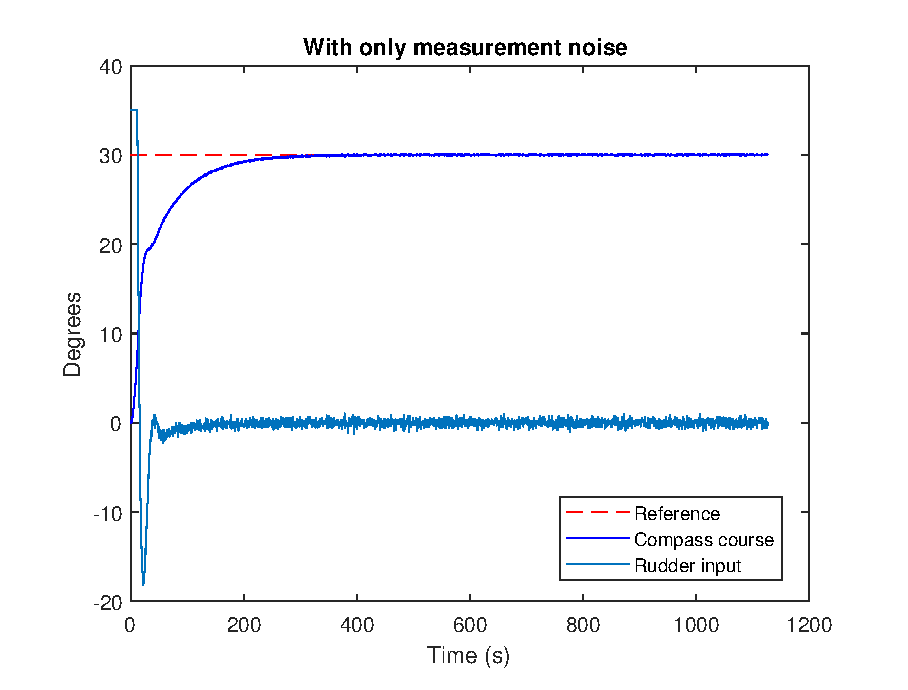
\includegraphics[width=0.5\linewidth]{Part3_pics/3b.eps}
    \caption{Compass compared to the reference}
    \label{sim:5.3.b}
\end{figure}



\newpage
\section{Plots}
\subsection{Part ...}